% Preview of the Experiment 1 network appendix (networks.py). Preamble: the packages of the thesis's
% dissertation.tex that tables and figures use (uathesis print layout: A4, 12 pt, scale 0.75,
% 5 mm binding offset), as thesis/ch7/exp1/preview.tex. algorithm.sty is omitted (not installed here).
%   cd thesis/ch7/exp1 && latexmk -pdf preview_networks.tex && latexmk -c preview_networks.tex
\documentclass[a4paper,12pt,openany]{book}
\usepackage[a4paper,hmarginratio=1:1,vmarginratio=1:1,scale=0.75,bindingoffset=5mm]{geometry}
\usepackage{graphicx}
\usepackage{cmap}
\usepackage{amssymb}
\usepackage{amsmath}
\usepackage{setspace}
\usepackage{booktabs}
\usepackage{url}
\usepackage{adjustbox}
\usepackage{tabularx}
\usepackage{tabularray}
\usepackage{multicol}
\usepackage{subcaption}
\usepackage[inline]{enumitem}
\usepackage[table,usenames,dvipsnames]{xcolor}
\usepackage[figuresright]{rotating}  % thesis: figuresright keeps multi-page sideways floats facing one way
\usepackage{makecell}
\usepackage[unicode=true,colorlinks=true,linkcolor=black]{hyperref}
\usepackage{cleveref}
% thesis-tablestyle.tex -- one table style for the whole thesis (every chapter, generated or hand-written).
%
% Load ONCE in the preamble, after xcolor (with its `table' option) and booktabs:
%     \usepackage[table,usenames,dvipsnames]{xcolor}   % already in dissertation.tex
%     \usepackage{booktabs}                            % already in dissertation.tex
%     \input{thesis-tablestyle}
%
% What it does, in every table / table* / sidewaystable / sidewaystable* float:
%   * zebra striping of the body rows (header rows stay white), in a very light grey that prints in greyscale;
%   * slightly taller rows (\arraystretch times \thesisrowstretch, on top of any \arraystretch the table sets);
%   * booktabs rules keep their spacing; where a rule follows a shaded row, the gap above the rule is shaded
%     too, so there is no white band.
% The body starts after the first \midrule (booktabs) or the second \hline (\hline tables). Striping restarts
% after every \midrule, so a group row after a \midrule (e.g. "\multicolumn{8}{l}{\textit{PropNEAT}}") is
% white and its rows alternate below it. A table whose header ends without a \midrule says how many header
% rows it has: \thesistablestyle[1]. A table with no top rule (\toprule or \hline) is not striped.
%
% Switches (in the preamble for the whole thesis, or inside one table for that table):
%   \thesisstripestrue / \thesisstripesfalse        zebra on (default) / off
%   \thesisfiverulestrue / \thesisfiverulesfalse    thin grey rule every \thesisfiveevery body rows (default off);
%                                                   the alternative to stripes: \thesisstripesfalse\thesisfiverulestrue
%   \thesistablesautotrue / \thesistablesautofalse  apply to every table float automatically (default on); when
%                                                   off, only tables that call \thesistablestyle are styled
%   \renewcommand\thesisrowstretch{1.1}             row-height factor (1 = unchanged)
%   \renewcommand\thesisfiveevery{5}                rows between the thin rules
%   \definecolor{thesisstripe}{gray}{0.93}          stripe colour (and thesisfiverule for the thin rules)
% Per table:
%   \thesistablestyle[<n>]   apply the style (generated tables call it first; idempotent); <n> = number of
%                            header rows after \toprule when the header does not end with a \midrule
%   \thesisnostripes         opt out: this table keeps its own look (no stripes, no thin rules, no extra
%                            height). Use it for tables that colour their own cells or rows, or use \multirow
%                            (the next row's shading would cover the \multirow text).
% Nested tabulars (\makecell, a tabular inside a cell) are left alone and do not disturb the outer striping.
\makeatletter
\@ifpackageloaded{colortbl}{}{\RequirePackage{colortbl}}
\@ifpackageloaded{booktabs}{}{\RequirePackage{booktabs}}
\@ifundefined{fpeval}{\RequirePackage{xfp}}{}

\newif\ifthesisstripes   \thesisstripestrue
\newif\ifthesisfiverules \thesisfiverulesfalse
\newif\ifthesistablesauto \thesistablesautotrue
\definecolor{thesisstripe}{gray}{0.93}
\definecolor{thesisfiverule}{gray}{0.6}
\newcommand\thesisrowstretch{1.1}
\newcommand\thesisfiveevery{5}

\newif\ifthesis@active   % inside a styled float
\newif\ifthesis@engine   % stripes or thin rules are being drawn
\newif\ifthesis@data     % past the header
\newif\ifthesis@firstrule
\newif\ifthesis@lastrow  % the last item was a row (not a rule)
\newif\ifthesis@curgrey  % the current row is shaded
\newif\ifthesis@lastgrey % the row just ended was shaded
\newif\ifthesis@wantsep
\newif\ifthesis@oksep
\newcount\thesis@row     % body row number since the last \midrule (1 = first)
\newcount\thesis@five
\newcount\thesis@head    % header rows still to come (-1: wait for a \midrule)
\newcount\thesis@lvl     % group level of the outer table's \noalign (-1: unknown)
\thesis@lvl=\m@ne
\def\thesis@headrows{-1}

% ---- row colours (colortbl's per-row colour, as xcolor's \rowcolors sets it). colortbl extends each
% cell's colour by \tabcolsep on both sides; at an @{} edge that would stick out past the rules, so the
% first / last cell of a row drops that overhang when the column spec starts / ends with @{}.
\newif\ifthesis@leftflush
\newif\ifthesis@rightflush
\newcount\thesis@cellno
\newcount\thesis@ncols
% colortbl stretches a cell's colour with 1fill against the cell's own 1fill of alignment glue; a
% \makecell adds its own \hfill glue (counted in \thesis@mc), which would take part of the stretch and
% leave the right of the cell white. The colour's stretch is raised to match (\thesis@k).
\newcount\thesis@mc
\def\thesis@k{1}
\def\thesis@mcell#1#2\@nil#3{\thesis@o@mcell{#1}#2\@nil{#3}%
  \ifx\mcell@left\hfill\global\advance\thesis@mc\@ne\fi
  \ifx\mcell@right\hfill\global\advance\thesis@mc\@ne\fi}
\def\thesis@docolor{\global\let\CT@do@color\relax
  \@tempdima\wd\z@\advance\@tempdima\@tempdimb\advance\@tempdima\@tempdimc
  \kern-\@tempdimb\leaders\vrule\hskip\@tempdima\@plus\thesis@k fill
  \kern-\@tempdimc\hskip-\wd\z@\@plus-\thesis@k fill\relax}
\def\thesis@cellstep{%
  \def\thesis@k{1}%
  \ifnum\currentgrouplevel=\thesis@lvl
    \edef\thesis@k{\the\numexpr\@ne+\thesis@mc\relax}\global\thesis@mc\z@
    \global\advance\thesis@cellno\@ne
    % overlap the next cell a little, so screen renderers show no hairline gaps between cells
    \ifnum\thesis@cellno<\thesis@ncols\advance\@tempdimc.25pt\fi
    \ifnum\thesis@cellno=\@ne\ifthesis@leftflush\@tempdimb\z@\fi\fi
    \ifnum\thesis@cellno=\thesis@ncols\ifthesis@rightflush\@tempdimc\z@\fi\fi
  \fi}
\def\thesis@grey{\gdef\CT@row@color{\thesis@cellstep\CT@color{thesisstripe}}\global\thesis@curgreytrue}
\def\thesis@white{\gdef\CT@row@color{\thesis@cellstep}\global\thesis@curgreyfalse}
\ExplSyntaxOn
\cs_new_protected:Npn \thesis@edges #1
  {
    \str_set:Nn \l_tmpa_str {#1}
    \str_remove_all:Nn \l_tmpa_str { ~ }
    \str_if_eq:eeTF { \str_head:N \l_tmpa_str } { @ }
      { \global\thesis@leftflushtrue } { \global\thesis@leftflushfalse }
    \str_if_eq:eeTF { \str_range:Nnn \l_tmpa_str { -3 } { -1 } } { \tl_to_str:n { @{} } }
      { \global\thesis@rightflushtrue } { \global\thesis@rightflushfalse }
  }
\ExplSyntaxOff
\def\thesis@array[#1]#2{%
  \ifnum\thesis@lvl<\z@\thesis@edges{#2}\else\ifnum\currentgrouplevel<\thesis@lvl\thesis@edges{#2}\fi\fi
  \thesis@o@array[#1]{#2}}
\def\thesis@colour{\ifthesisstripes\ifodd\thesis@row\thesis@white\else\thesis@grey\fi\else\thesis@white\fi}
\def\thesis@startdata{\global\thesis@datatrue\global\thesis@head\m@ne\global\thesis@row\@ne
  \global\thesis@five\z@\thesis@colour}
\def\thesis@sethead{\global\thesis@lvl\currentgrouplevel\global\thesis@firstrulefalse
  \global\thesis@ncols\z@\global\thesis@cellno\z@
  \global\thesis@datafalse\global\thesis@row\z@\global\thesis@five\z@\thesis@white
  \global\thesis@head=\thesis@headrows\relax\ifnum\thesis@head=\z@\thesis@startdata\fi}

% ---- at every row end (\CT@everycr); only the outer table's rows count
\def\thesis@close{\ifnum0=`{\fi}}
\def\thesis@cr{\noalign{\ifnum0=`}\fi\thesis@crstep}
\def\thesis@crstep{\thesis@wantsepfalse
  \ifnum\currentgrouplevel=\thesis@lvl
    \ifthesis@curgrey\global\thesis@lastgreytrue\else\global\thesis@lastgreyfalse\fi
    \global\thesis@lastrowtrue
    \ifnum\thesis@cellno>\thesis@ncols\global\thesis@ncols\thesis@cellno\fi
    \global\thesis@cellno\z@\global\thesis@mc\z@
    \ifthesis@data
      \global\advance\thesis@row\@ne\thesis@colour
      \ifthesisfiverules
        \global\advance\thesis@five\@ne
        \ifnum\thesis@five<\thesisfiveevery\relax\else\global\thesis@five\z@\thesis@wantseptrue\fi
      \fi
    \else
      \thesis@white
      \ifnum\thesis@head>\z@
        \global\advance\thesis@head\m@ne
        \ifnum\thesis@head=\z@\thesis@startdata\fi
      \fi
    \fi
  \fi
  \ifthesis@wantsep\expandafter\thesis@peek\else\expandafter\thesis@close\fi}
% a thin rule after every \thesisfiveevery body rows, unless a rule or the end comes next
\def\thesis@peek{\futurenonspacelet\thesis@next\thesis@decide}
\def\thesis@nosepif#1{\ifx\thesis@next#1\thesis@oksepfalse\fi}
\def\thesis@decide{\thesis@okseptrue
  \thesis@nosepif\bottomrule\thesis@nosepif\midrule\thesis@nosepif\toprule\thesis@nosepif\cmidrule
  \thesis@nosepif\hline\thesis@nosepif\cline\thesis@nosepif\addlinespace\thesis@nosepif\specialrule
  \thesis@nosepif\end\thesis@nosepif\noalign\thesis@nosepif\crcr
  \ifthesis@oksep{\color{thesisfiverule}\hrule\@height\cmidrulewidth}\fi
  \thesis@close}

% ---- rules: #1 = 0 \cmidrule, 1 \toprule, 2 \midrule, 3 \bottomrule, 4 \hline
\def\thesis@fill{{\color{thesisstripe}\hrule\@height\aboverulesep}\vskip-\aboverulesep}
\def\thesis@rule#1{\noalign{\thesis@rulestep#1}}
\def\thesis@rulestep#1{%
  \ifnum#1=\@ne\thesis@sethead\else
  \ifnum#1=4
    \ifthesis@firstrule\thesis@sethead\else
    \ifnum\currentgrouplevel=\thesis@lvl\thesis@startdata\else\thesis@sethead\fi\fi
  \else
  \ifnum\currentgrouplevel=\thesis@lvl
    \ifthesis@lastrow\ifthesis@lastgrey\thesis@fill\fi\fi
    \ifnum#1=\tw@\thesis@startdata\fi
    \ifnum#1=\thr@@\global\thesis@datafalse\thesis@white\fi
  \fi\fi\fi
  \global\thesis@lastrowfalse}

% ---- at the start of each tabular / tabularx / tabular* (not nested ones): reset, taller rows
\def\thesis@tabbegin{%
  \ifthesis@active
    \ifnum\thesis@lvl<\z@\thesis@tabreset\else
    \ifnum\currentgrouplevel<\thesis@lvl\thesis@tabreset\fi\fi
  \fi}
\def\thesis@tabreset{\global\thesis@lvl\m@ne\global\thesis@firstruletrue\global\thesis@datafalse
  \global\thesis@row\z@\global\thesis@five\z@\global\thesis@head\m@ne\global\thesis@lastrowfalse
  \global\thesis@curgreyfalse
  \edef\arraystretch{\fpeval{\arraystretch*\thesisrowstretch}}}
\AddToHook{env/tabular/begin}{\thesis@tabbegin}
\AddToHook{env/tabular*/begin}{\thesis@tabbegin}
\AddToHook{env/tabularx/begin}{\thesis@tabbegin}

% ---- the style itself
\newcommand\thesistablestyle[1][-1]{%
  \def\thesis@headrows{#1}%
  \ifthesis@active\else
    \thesis@activetrue\global\thesis@lvl\m@ne
    \thesis@enginefalse
    \ifthesisstripes\thesis@enginetrue\fi
    \ifthesisfiverules\thesis@enginetrue\fi
    \ifthesis@engine
      \CT@everycr{\the\everycr\thesis@cr}%
      \let\thesis@o@toprule\toprule\def\toprule{\thesis@rule1\thesis@o@toprule}%
      \let\thesis@o@midrule\midrule\def\midrule{\thesis@rule2\thesis@o@midrule}%
      \let\thesis@o@bottomrule\bottomrule\def\bottomrule{\thesis@rule3\thesis@o@bottomrule}%
      \let\thesis@o@cmidrule\cmidrule\def\cmidrule{\thesis@rule0\thesis@o@cmidrule}%
      \let\thesis@o@hline\hline\def\hline{\thesis@rule4\thesis@o@hline}%
      \ifdefined\@@array\let\thesis@o@array\@@array\let\@@array\thesis@array\fi
      \ifdefined\mcell@@@tabular\let\thesis@o@mcell\mcell@@@tabular\let\mcell@@@tabular\thesis@mcell\fi
      \let\thesis@o@docolor\CT@@do@color\let\CT@@do@color\thesis@docolor
    \fi
  \fi}
\newcommand\thesisnostripes{%
  \ifthesis@active
    \thesis@activefalse
    \ifthesis@engine
      \CT@everycr{\noalign{\global\let\CT@row@color\relax}\the\everycr}%
      \let\toprule\thesis@o@toprule\let\midrule\thesis@o@midrule\let\bottomrule\thesis@o@bottomrule
      \let\cmidrule\thesis@o@cmidrule\let\hline\thesis@o@hline
      \ifdefined\thesis@o@array\let\@@array\thesis@o@array\fi
      \ifdefined\thesis@o@mcell\let\mcell@@@tabular\thesis@o@mcell\fi
      \let\CT@@do@color\thesis@o@docolor
      \thesis@enginefalse
    \fi
  \fi}
\def\thesis@auto{\ifthesistablesauto\thesistablestyle\fi}
\AddToHook{env/table/begin}{\thesis@auto}
\AddToHook{env/table*/begin}{\thesis@auto}
\AddToHook{env/sidewaystable/begin}{\thesis@auto}
\AddToHook{env/sidewaystable*/begin}{\thesis@auto}
\makeatother
  % thesis table style (loaded once in the thesis preamble)
\graphicspath{{./}{../figures/}}            % figures/exp1/networks here; figures/ch7/appendix under ../figures
\newcolumntype{Y}{>{\centering\arraybackslash}X}
\renewcommand\floatpagefraction{.9}
\renewcommand\topfraction{.9}
\renewcommand\bottomfraction{.9}
\renewcommand\textfraction{.1}
\setcounter{totalnumber}{50}
\setcounter{topnumber}{50}
\setcounter{bottomnumber}{50}
\begin{document}
\appendix
\chapter{Chapter 7 appendix}
% Generated by thesis/ch7/exp1/networks.py -- do not edit by hand.
% Appendix: Experiment 1 networks, as trained and as explained.
% Picture height: 0.9 of the portrait text width, fixed here (inside a sidewaysfigure \textwidth is the
% page's long side).
\ifdefined\netfigheight\else\newlength{\netfigheight}\setlength{\netfigheight}{0.9\textwidth}\fi
% Spreads: a case's heading on a right (odd) page, its raw network on the left (even) page after it and
% the explained network facing it on the right.
\providecommand{\cleartoevenpage}{\clearpage\ifodd\value{page}\hbox{}\thispagestyle{empty}\newpage\fi}
\providecommand{\cleartooddpage}{\clearpage\ifodd\value{page}\else\hbox{}\thispagestyle{empty}\newpage\fi}
\section{Experiment 1 networks}\label{app:exp1-networks}
% Adult, original network
\cleartooddpage
\subsection{Adult}\label{app:exp1-net-adult}
\cleartoevenpage
\begin{sidewaysfigure}
  \centering
  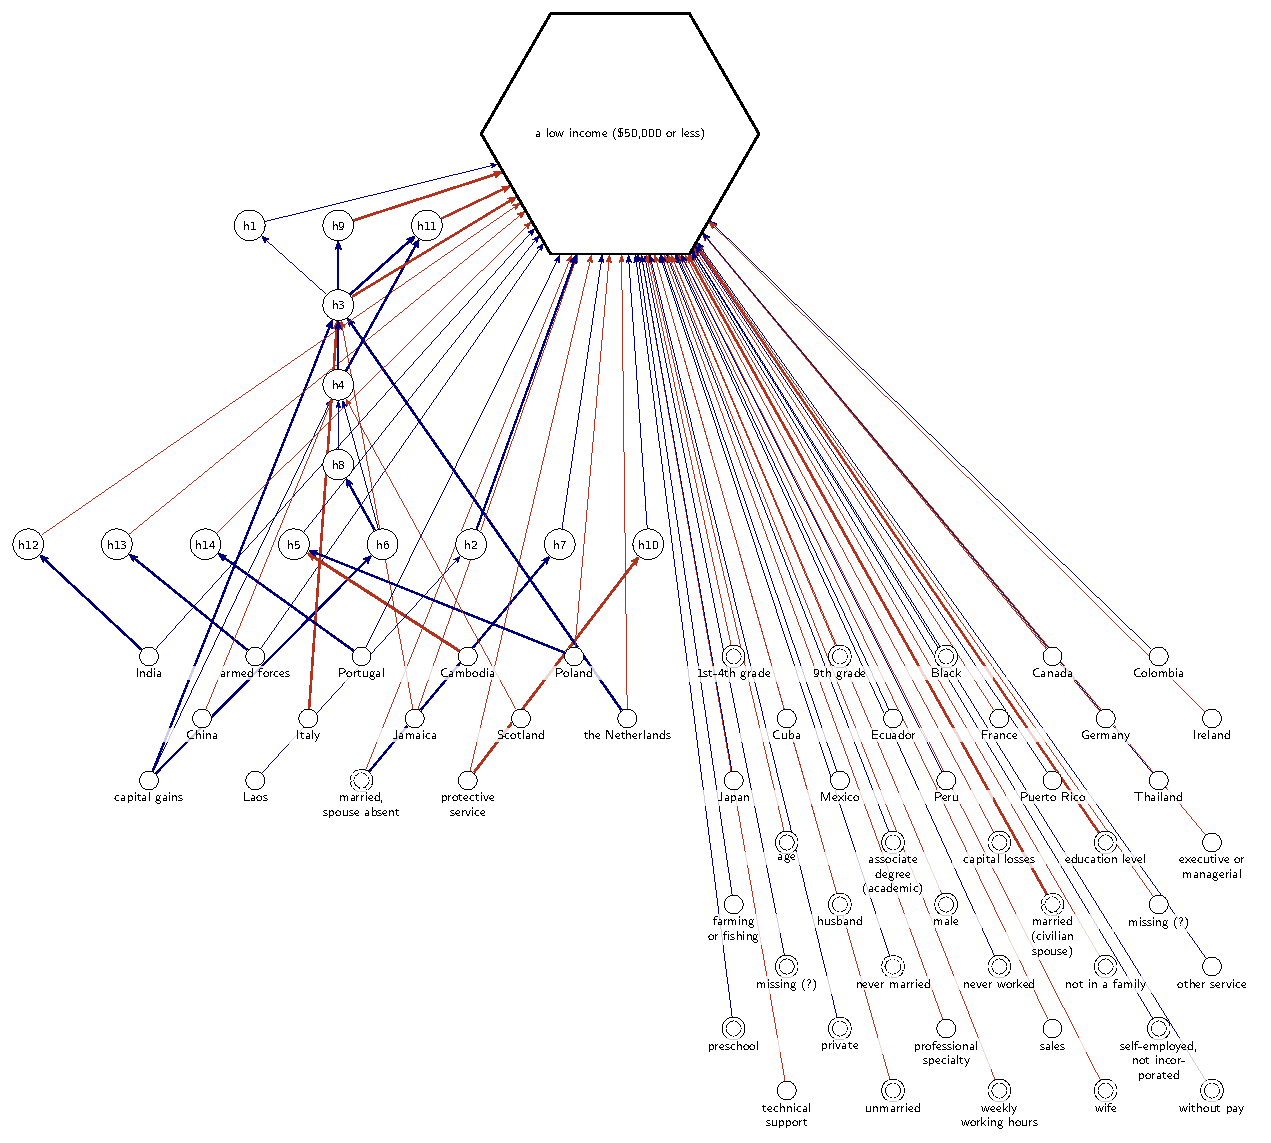
\includegraphics[width=\textheight,height=\netfigheight,keepaspectratio]{figures/exp1/networks/paper-adult-raw}
  \caption{Adult, original network: the network as trained, before any explanation. Bottom: the input columns; circles h1, h2, \ldots: hidden units; hexagon: the output. Edges: blue, a positive weight (raises the score); red, a negative weight (lowers it); thicker, a larger weight. Double outline: acts at a fixed rate everywhere (dashed double: on the observed data).}
  \label{fig:exp1-net-paper-adult-raw}
\end{sidewaysfigure}
\clearpage
\begin{sidewaysfigure}
  \centering
  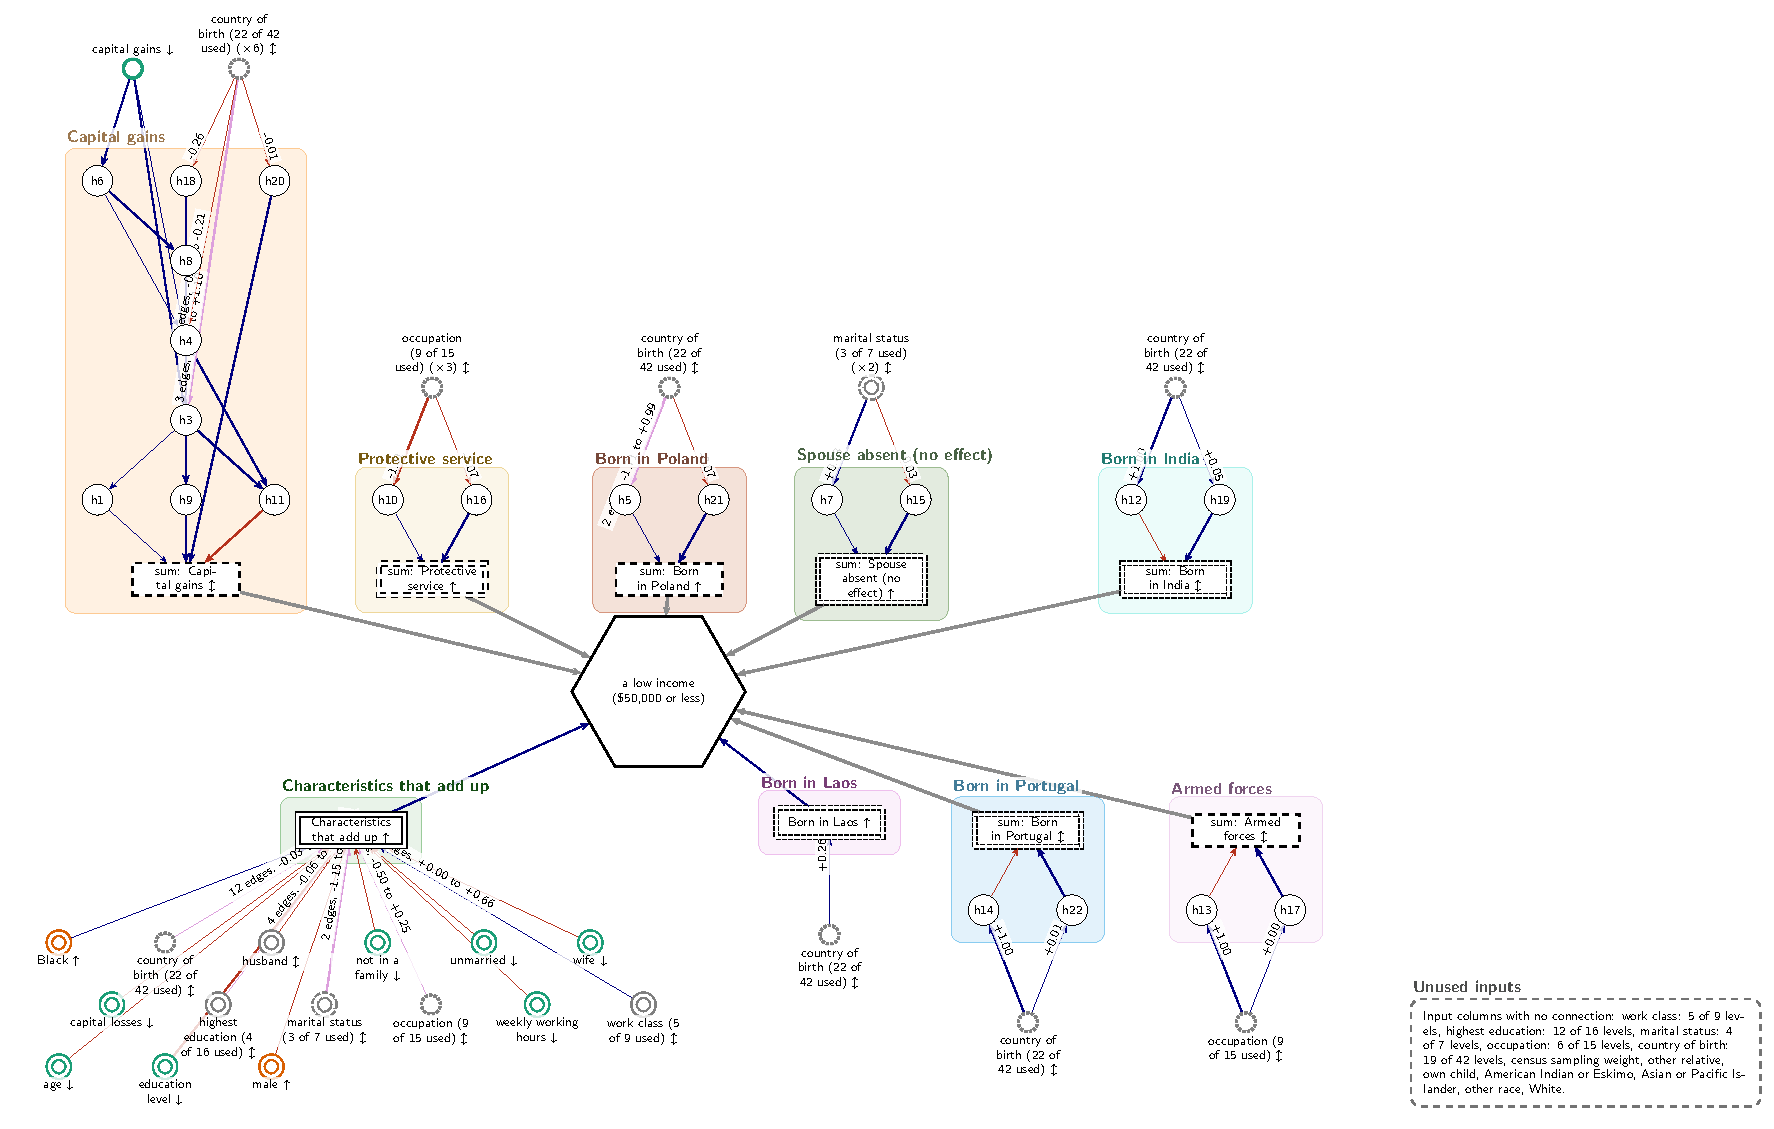
\includegraphics[width=\textheight,height=\netfigheight,keepaspectratio]{figures/exp1/networks/paper-adult-explained}
  \caption{Adult, original network: the explained network, every unit nested by part. Shaded boxes: the explanation's parts (inner boxes: sub-parts); white box: a part's output (dashed: a sum standing for the output unit's addition, grey edge). Each input is drawn under every part that reads it (dotted outline, $\times n$: read by $n$ parts); a variable with many levels is drawn once, its edges labelled with their number and weight range (purple: both signs). Orange outline and up arrow: raises the final prediction; teal and down arrow: lowers it; grey and double arrow: depends. Double outline: acts at a fixed rate everywhere (dashed double: on the observed data). Edges as in Figure~\ref{fig:exp1-net-paper-adult-raw}. Dashed grey box, right: the annotation of the input columns with no connection, outside the root.}
  \label{fig:exp1-net-paper-adult-explained}
\end{sidewaysfigure}
\clearpage
\clearpage
% Heart, original network
\cleartooddpage
\subsection{Heart}\label{app:exp1-net-heart}
\cleartoevenpage
\begin{sidewaysfigure}
  \centering
  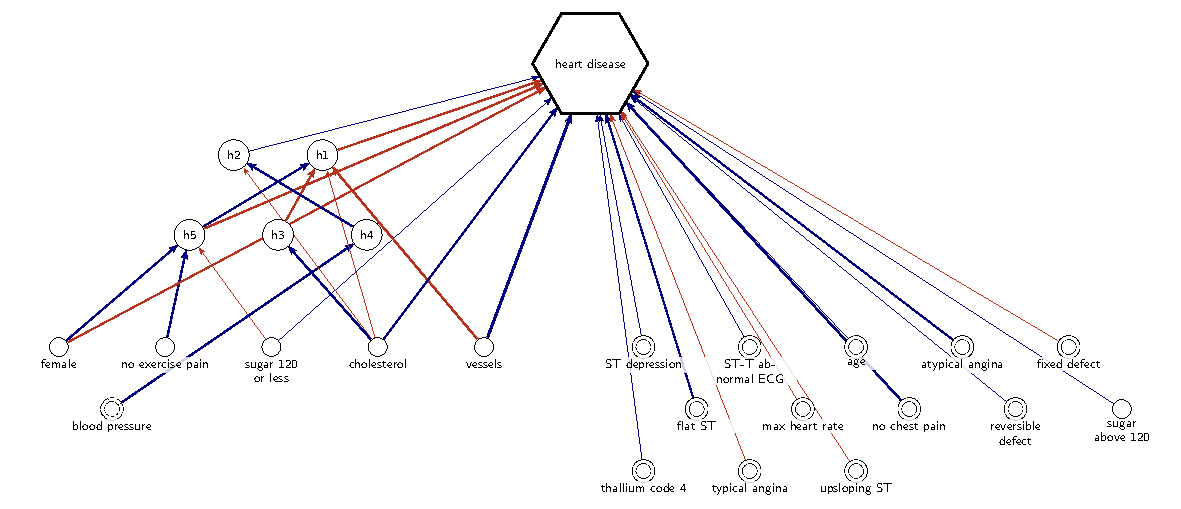
\includegraphics[width=\textheight,height=\netfigheight,keepaspectratio]{figures/exp1/networks/paper-heart-raw}
  \caption{Heart, original network: the network as trained, before any explanation. Bottom: the input columns; circles h1, h2, \ldots: hidden units; hexagon: the output. Edges: blue, a positive weight (raises the score); red, a negative weight (lowers it); thicker, a larger weight. Double outline: acts at a fixed rate everywhere (dashed double: on the observed data).}
  \label{fig:exp1-net-paper-heart-raw}
\end{sidewaysfigure}
\clearpage
\begin{sidewaysfigure}
  \centering
  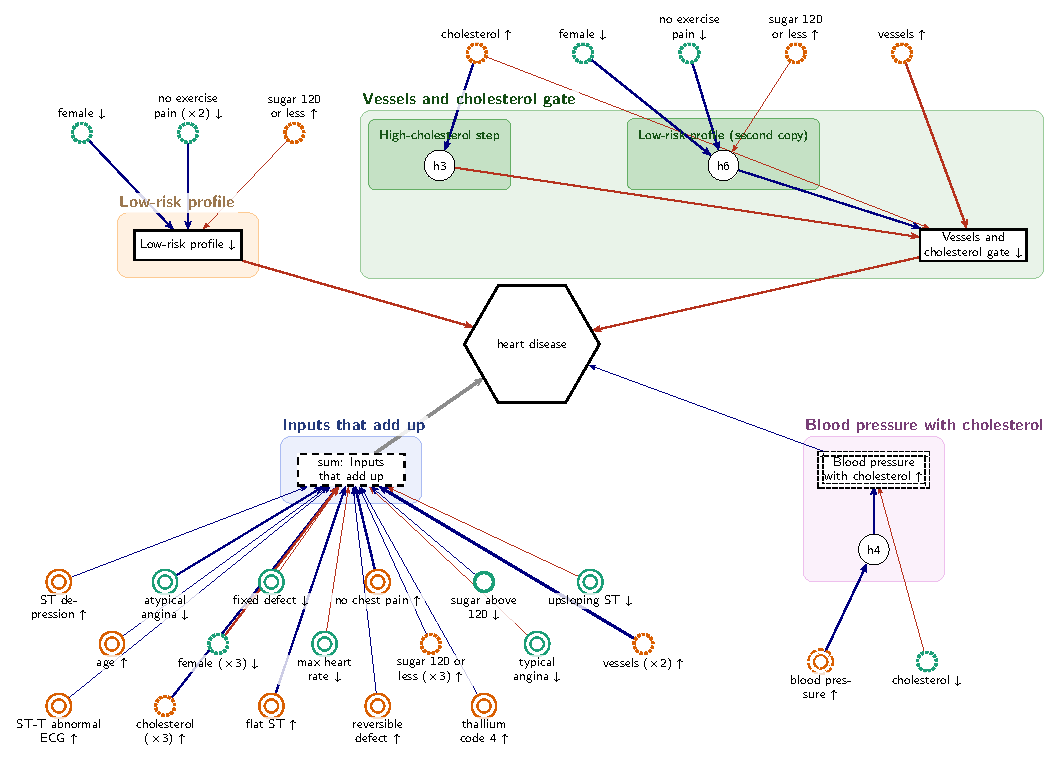
\includegraphics[width=\textheight,height=\netfigheight,keepaspectratio]{figures/exp1/networks/paper-heart-explained}
  \caption{Heart, original network: the explained network, every unit nested by part. Shaded boxes: the explanation's parts (inner boxes: sub-parts); white box: a part's output (dashed: a sum standing for the output unit's addition, grey edge). Each input is drawn under every part that reads it (dotted outline, $\times n$: read by $n$ parts); a variable with many levels is drawn once, its edges labelled with their number and weight range (purple: both signs). Orange outline and up arrow: raises the final prediction; teal and down arrow: lowers it; grey and double arrow: depends. Double outline: acts at a fixed rate everywhere (dashed double: on the observed data). Edges as in Figure~\ref{fig:exp1-net-paper-heart-raw}.}
  \label{fig:exp1-net-paper-heart-explained}
\end{sidewaysfigure}
\clearpage
\clearpage
% MONK-2, original network
\cleartooddpage
\subsection{MONK-2}\label{app:exp1-net-monk2}
\cleartoevenpage
\begin{sidewaysfigure}
  \centering
  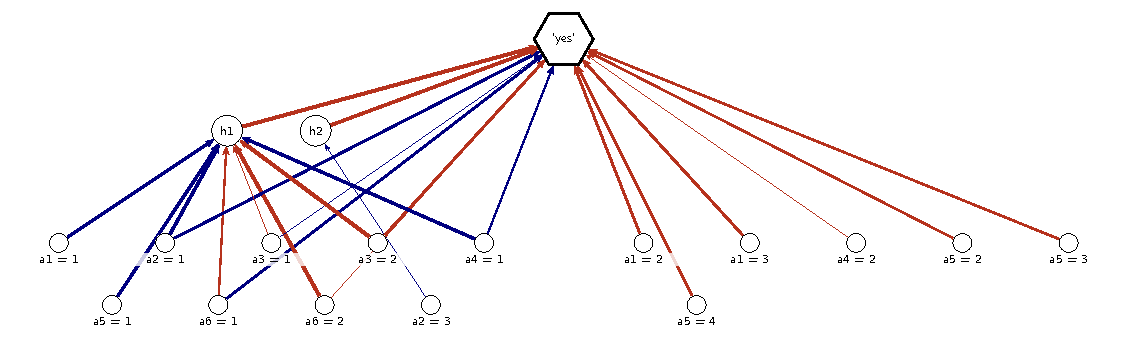
\includegraphics[width=\textheight,height=\netfigheight,keepaspectratio]{figures/exp1/networks/paper-monk2-raw}
  \caption{MONK-2, original network: the network as trained, before any explanation. Bottom: the input columns; circles h1, h2, \ldots: hidden units; hexagon: the output. Edges: blue, a positive weight (raises the score); red, a negative weight (lowers it); thicker, a larger weight. Double outline: acts at a fixed rate everywhere (dashed double: on the observed data).}
  \label{fig:exp1-net-paper-monk2-raw}
\end{sidewaysfigure}
\clearpage
\begin{sidewaysfigure}
  \centering
  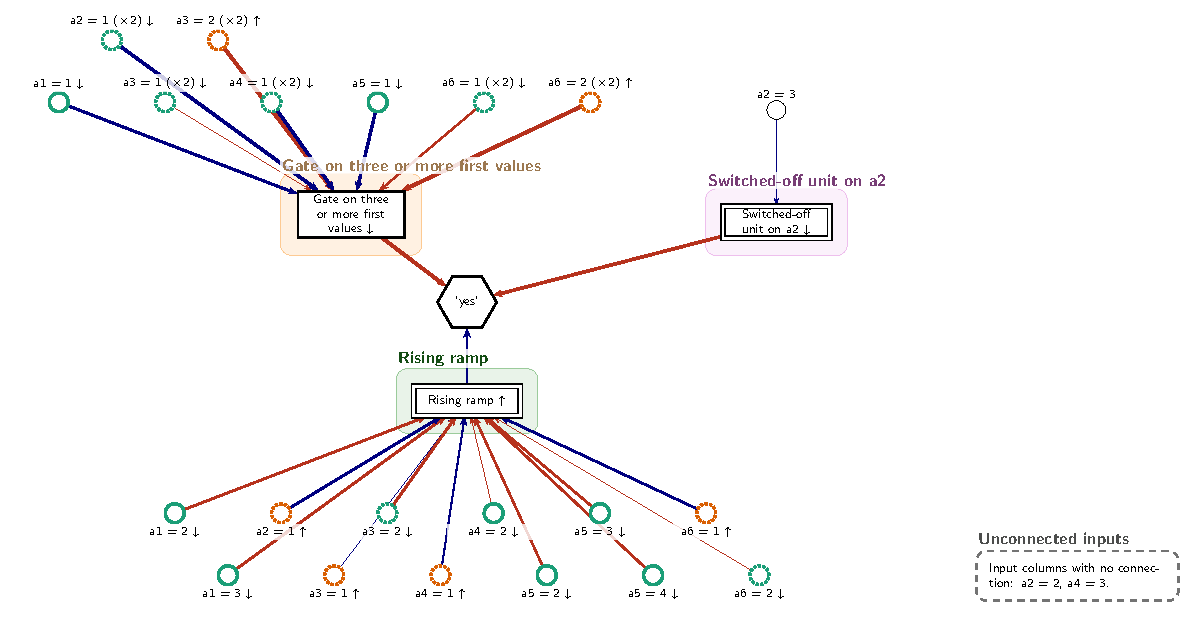
\includegraphics[width=\textheight,height=\netfigheight,keepaspectratio]{figures/exp1/networks/paper-monk2-explained}
  \caption{MONK-2, original network: the explained network, every unit nested by part. Shaded boxes: the explanation's parts (inner boxes: sub-parts); white box: a part's output (dashed: a sum standing for the output unit's addition, grey edge). Each input is drawn under every part that reads it (dotted outline, $\times n$: read by $n$ parts); a variable with many levels is drawn once, its edges labelled with their number and weight range (purple: both signs). Orange outline and up arrow: raises the final prediction; teal and down arrow: lowers it; grey and double arrow: depends. Double outline: acts at a fixed rate everywhere (dashed double: on the observed data). Edges as in Figure~\ref{fig:exp1-net-paper-monk2-raw}. Dashed grey box, right: the annotation of the input columns with no connection, outside the root.}
  \label{fig:exp1-net-paper-monk2-explained}
\end{sidewaysfigure}
\clearpage
\clearpage
% Churn, seed 10
\cleartooddpage
\subsection{Churn}\label{app:exp1-net-churn}
\cleartoevenpage
\begin{sidewaysfigure}
  \centering
  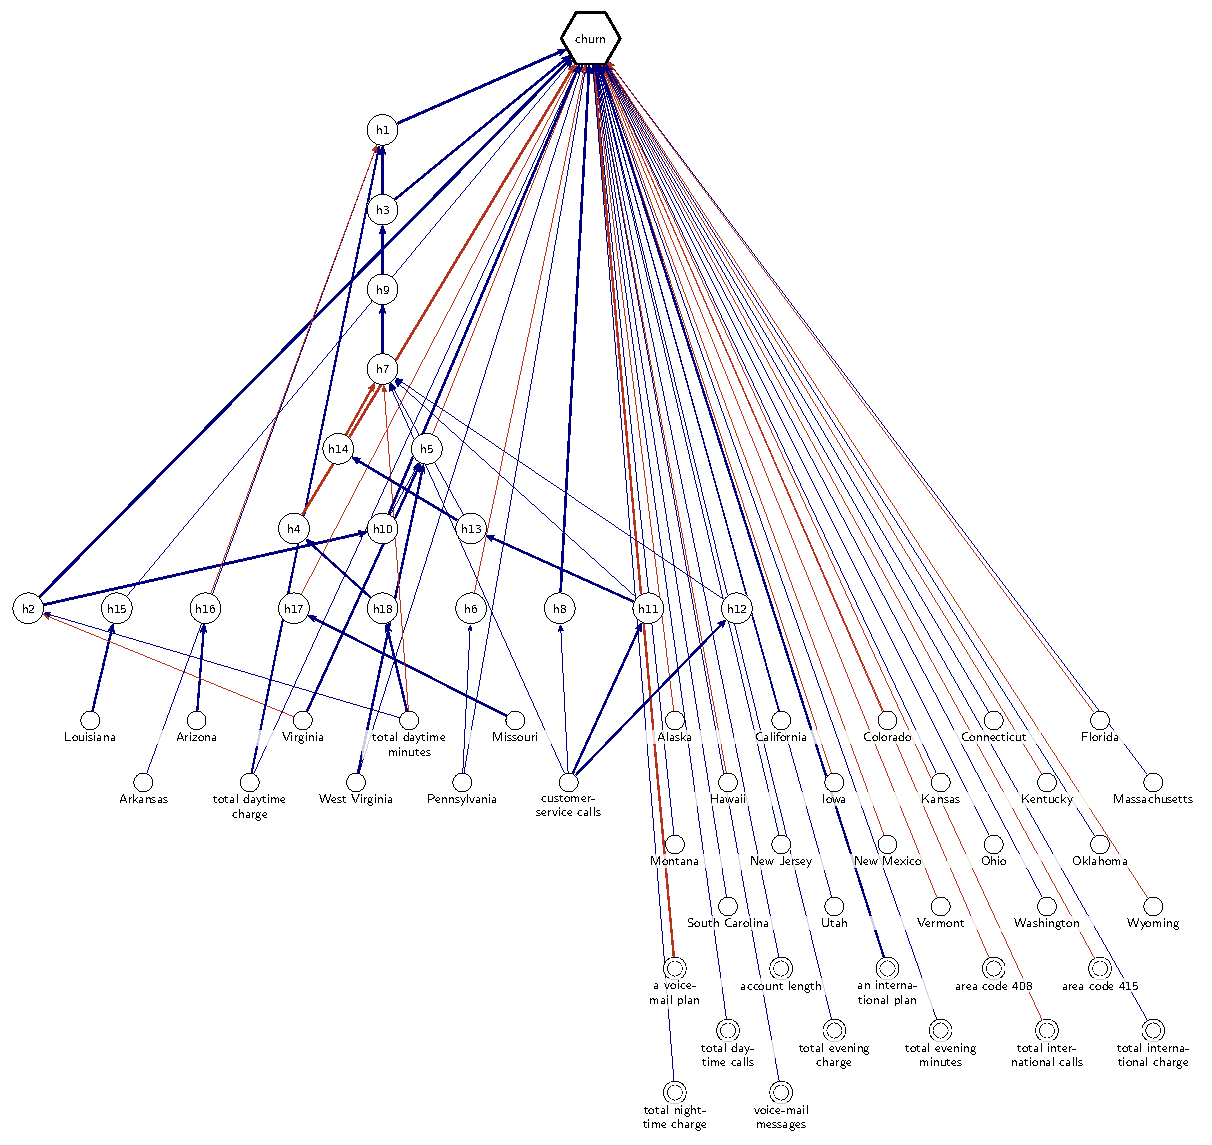
\includegraphics[width=\textheight,height=\netfigheight,keepaspectratio]{figures/exp1/networks/churn-case-s10-raw}
  \caption{Churn, seed 10: the network as trained, before any explanation. Bottom: the input columns; circles h1, h2, \ldots: hidden units; hexagon: the output. Edges: blue, a positive weight (raises the score); red, a negative weight (lowers it); thicker, a larger weight. Double outline: acts at a fixed rate everywhere (dashed double: on the observed data).}
  \label{fig:exp1-net-churn-case-s10-raw}
\end{sidewaysfigure}
\clearpage
\begin{sidewaysfigure}
  \centering
  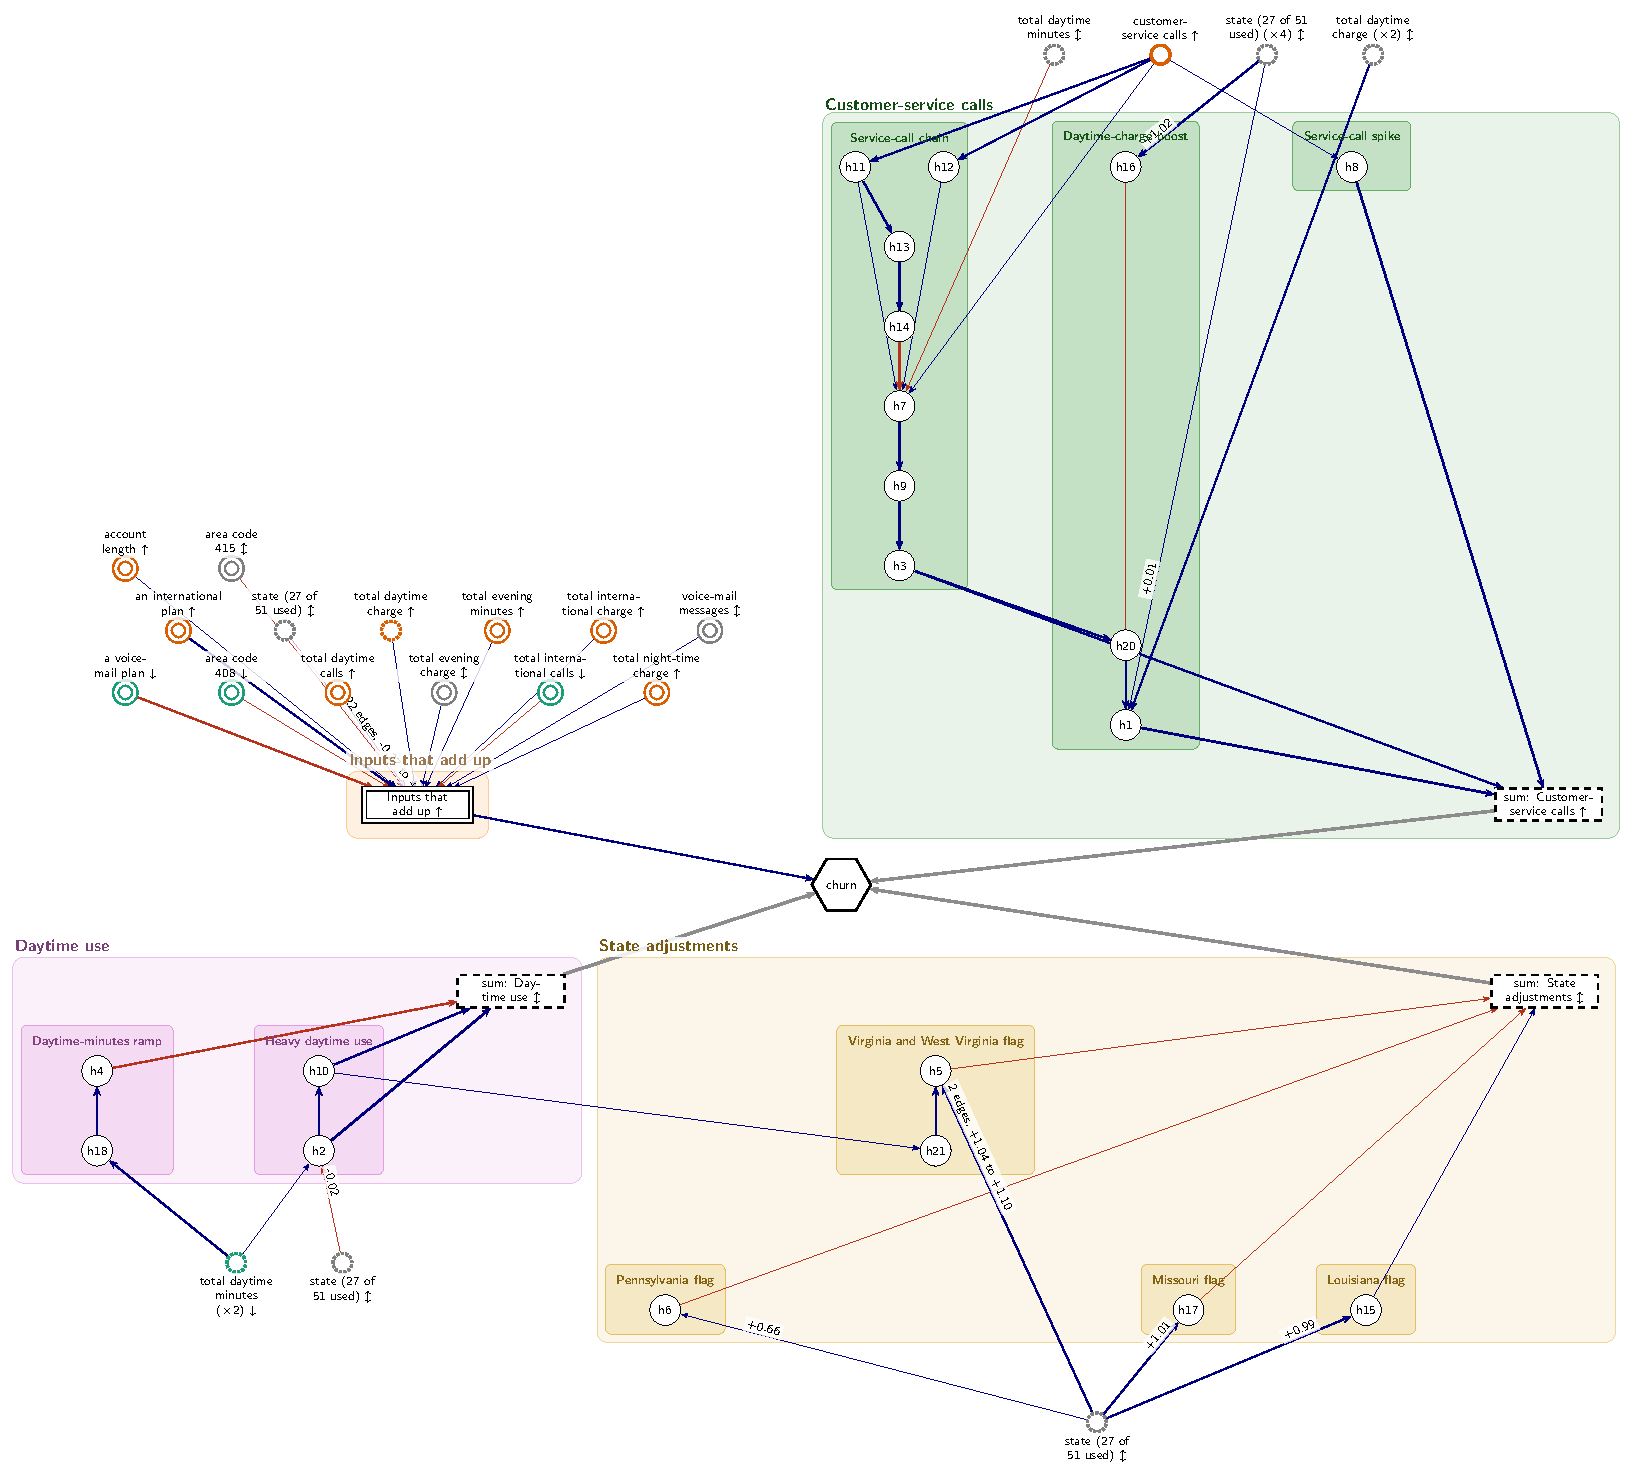
\includegraphics[width=\textheight,height=\netfigheight,keepaspectratio]{figures/exp1/networks/churn-case-s10-explained}
  \caption{Churn, seed 10: the explained network, every unit nested by part. Shaded boxes: the explanation's parts (inner boxes: sub-parts); white box: a part's output (dashed: a sum standing for the output unit's addition, grey edge). Each input is drawn under every part that reads it (dotted outline, $\times n$: read by $n$ parts); a variable with many levels is drawn once, its edges labelled with their number and weight range (purple: both signs). Orange outline and up arrow: raises the final prediction; teal and down arrow: lowers it; grey and double arrow: depends. Double outline: acts at a fixed rate everywhere (dashed double: on the observed data). Edges as in Figure~\ref{fig:exp1-net-churn-case-s10-raw}.}
  \label{fig:exp1-net-churn-case-s10-explained}
\end{sidewaysfigure}
\clearpage
\clearpage
% Connect-4, cells, seed 1
\cleartooddpage
\subsection{Connect-4, cells}\label{app:exp1-net-c4cells}
\begin{sidewaysfigure}
  \centering
  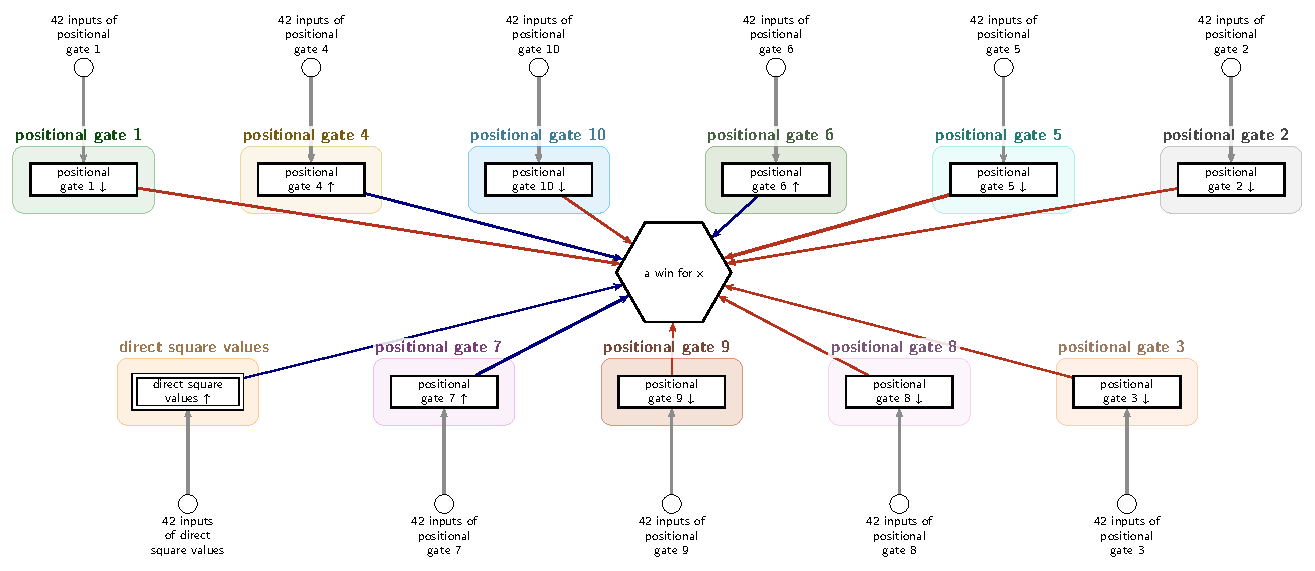
\includegraphics[width=\textheight,height=\netfigheight,keepaspectratio]{figures/exp1/networks/c4cap-main-h10-e50-s1-explained}
  \caption{Connect-4, cells, seed 1: the explained network, each top-level part collapsed into one box (its output), the inputs each part reads below it. Grey edges: the inputs a collapsed part reads (no single weight); a part reading many input columns has them drawn as one input. Arrows on inputs and boxes: the direction of the effect on the final prediction (up raises it, down lowers it, double arrow depends). Edges: blue, a positive weight (raises the score); red, a negative weight (lowers it); thicker, a larger weight.}
  \label{fig:exp1-net-c4cap-main-h10-e50-s1-explained}
\end{sidewaysfigure}
\clearpage
\clearpage
% Connect-4, lines, seed 0
\cleartooddpage
\subsection{Connect-4, lines}\label{app:exp1-net-c4lines}
\cleartoevenpage
\begin{sidewaysfigure}
  \centering
  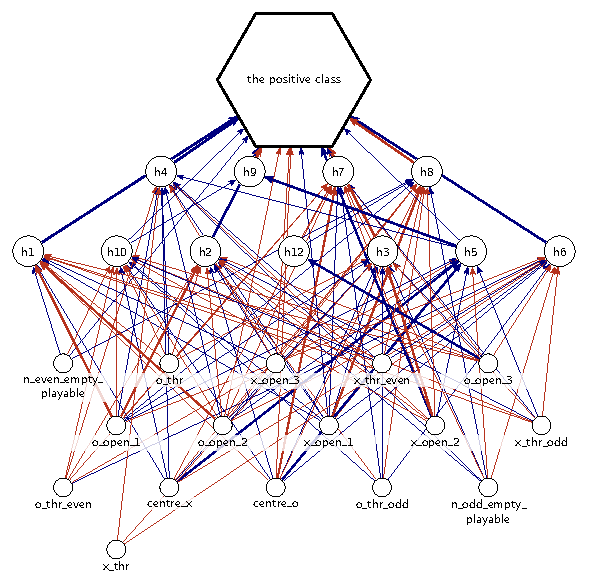
\includegraphics[width=\textheight,height=\netfigheight,keepaspectratio]{figures/exp1/networks/c4lf-lines-heavy-s0-raw}
  \caption{Connect-4, lines, seed 0: the network as trained, before any explanation. Bottom: the input columns; circles h1, h2, \ldots: hidden units; hexagon: the output. Edges: blue, a positive weight (raises the score); red, a negative weight (lowers it); thicker, a larger weight. Double outline: acts at a fixed rate everywhere (dashed double: on the observed data).}
  \label{fig:exp1-net-c4lf-lines-heavy-s0-raw}
\end{sidewaysfigure}
\clearpage
\begin{sidewaysfigure}
  \centering
  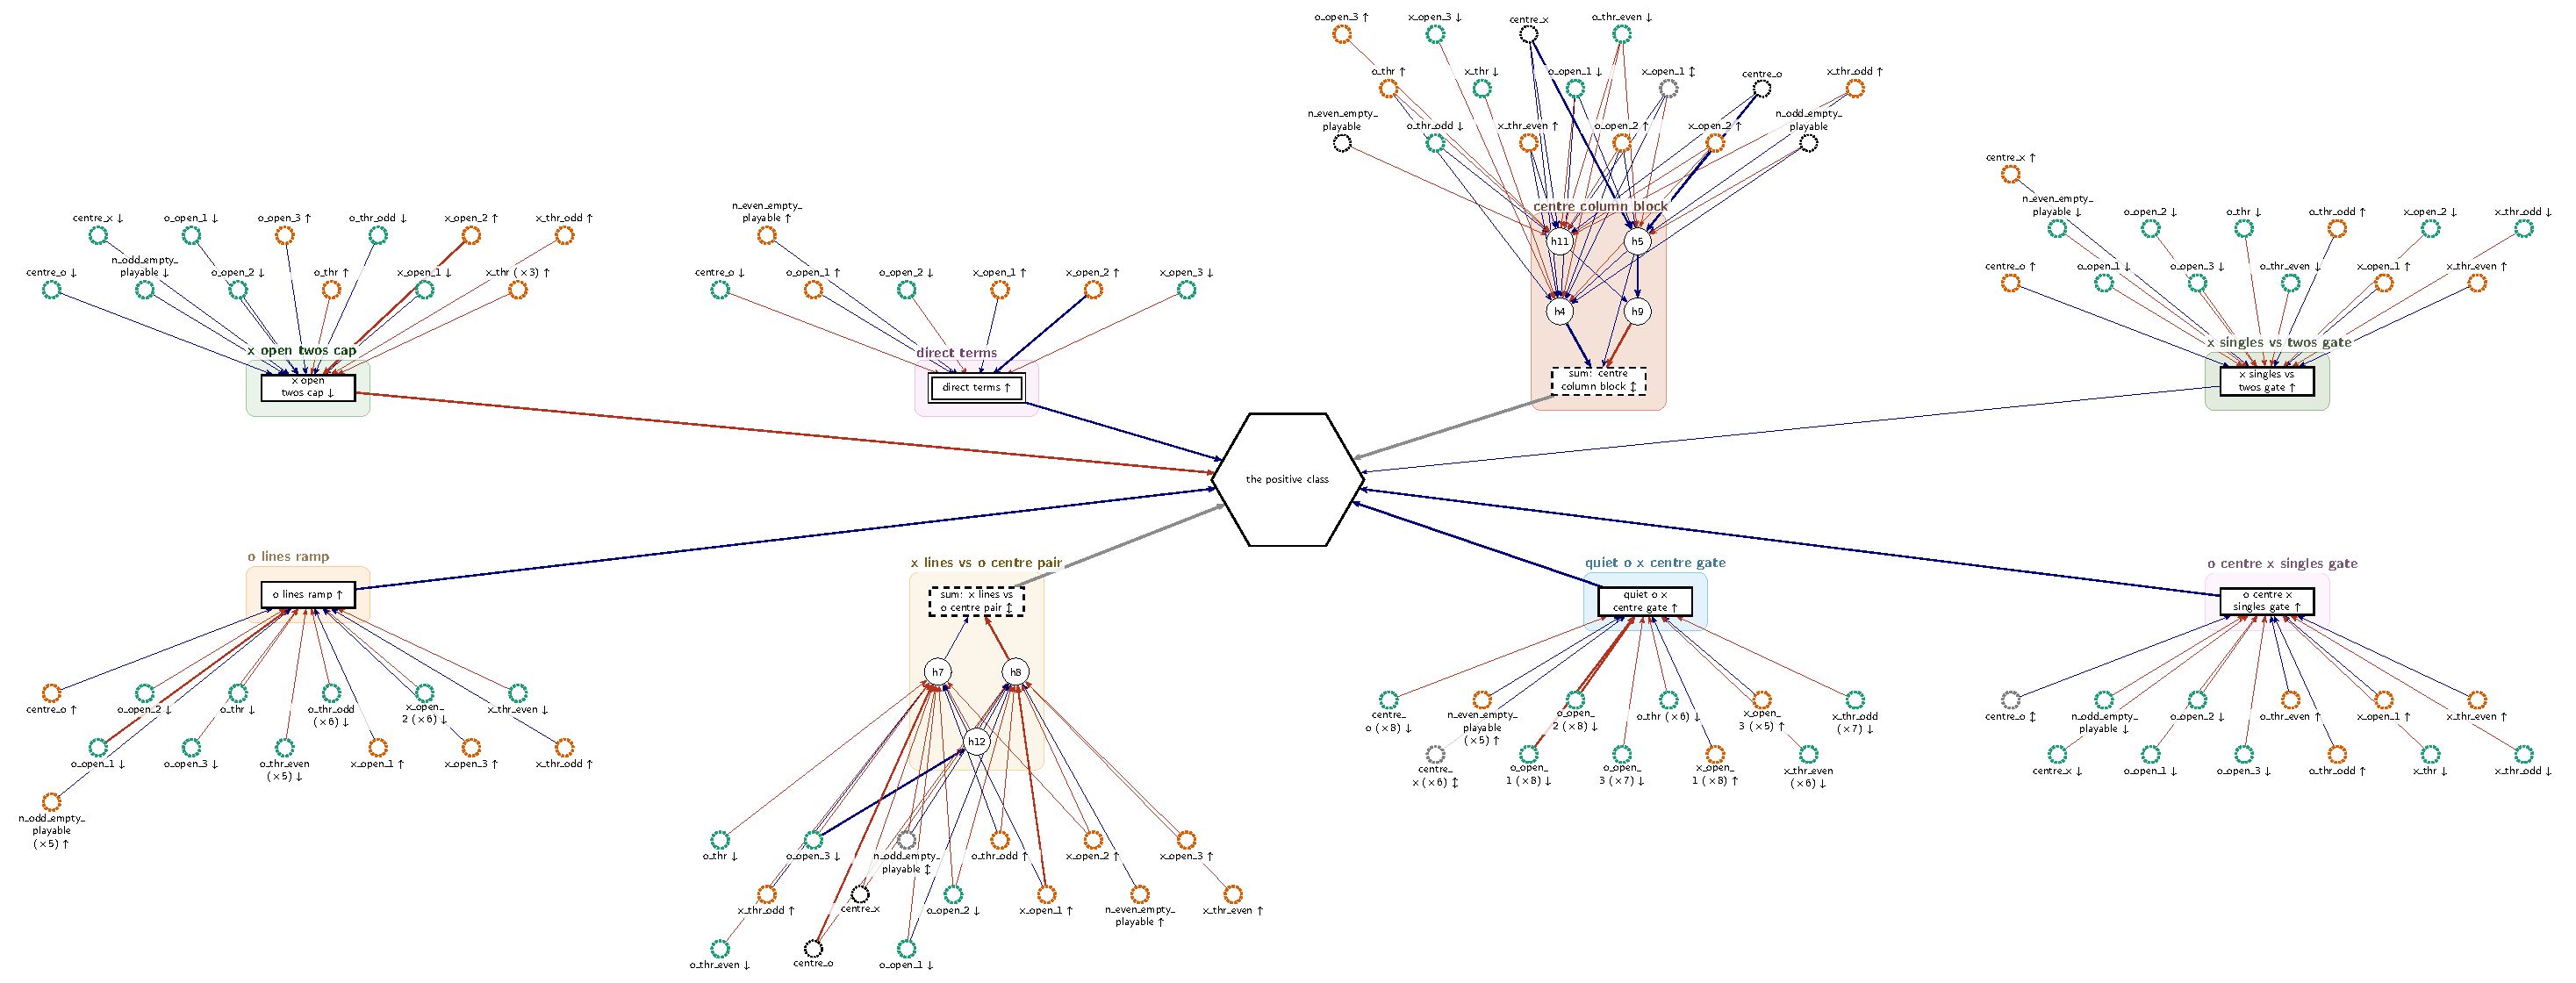
\includegraphics[width=\textheight,height=\netfigheight,keepaspectratio]{figures/exp1/networks/c4lf-lines-heavy-s0-explained}
  \caption{Connect-4, lines, seed 0: the explained network, each top-level part collapsed into one box (its output), the inputs each part reads below it. Grey edges: the inputs a collapsed part reads (no single weight); a part reading many input columns has them drawn as one input. Arrows on inputs and boxes: the direction of the effect on the final prediction (up raises it, down lowers it, double arrow depends). Edges: blue, a positive weight (raises the score); red, a negative weight (lowers it); thicker, a larger weight.}
  \label{fig:exp1-net-c4lf-lines-heavy-s0-explained}
\end{sidewaysfigure}
\clearpage
\clearpage
% Synthetic U and saddle, seed 4
\cleartooddpage
\subsection{Synthetic U and saddle}\label{app:exp1-net-shapeC}
\cleartoevenpage
\begin{sidewaysfigure}
  \centering
  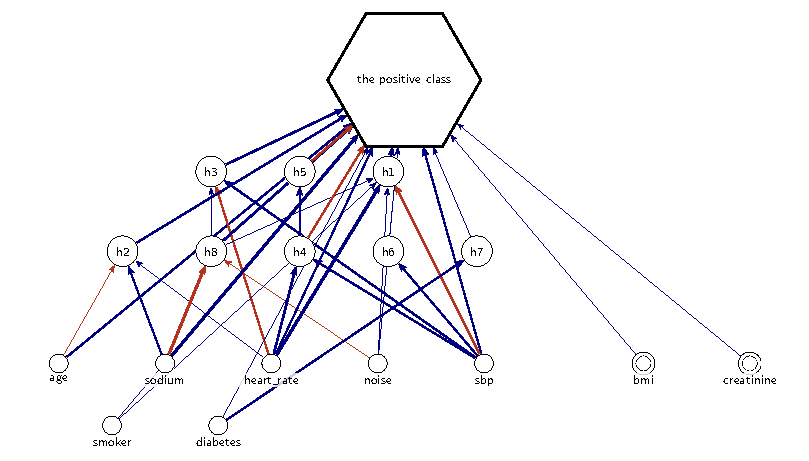
\includegraphics[width=\textheight,height=\netfigheight,keepaspectratio]{figures/exp1/networks/shape-C-raw}
  \caption{Synthetic U and saddle, seed 4: the network as trained, before any explanation. Bottom: the input columns; circles h1, h2, \ldots: hidden units; hexagon: the output. Edges: blue, a positive weight (raises the score); red, a negative weight (lowers it); thicker, a larger weight. Double outline: acts at a fixed rate everywhere (dashed double: on the observed data).}
  \label{fig:exp1-net-shape-C-raw}
\end{sidewaysfigure}
\clearpage
\begin{sidewaysfigure}
  \centering
  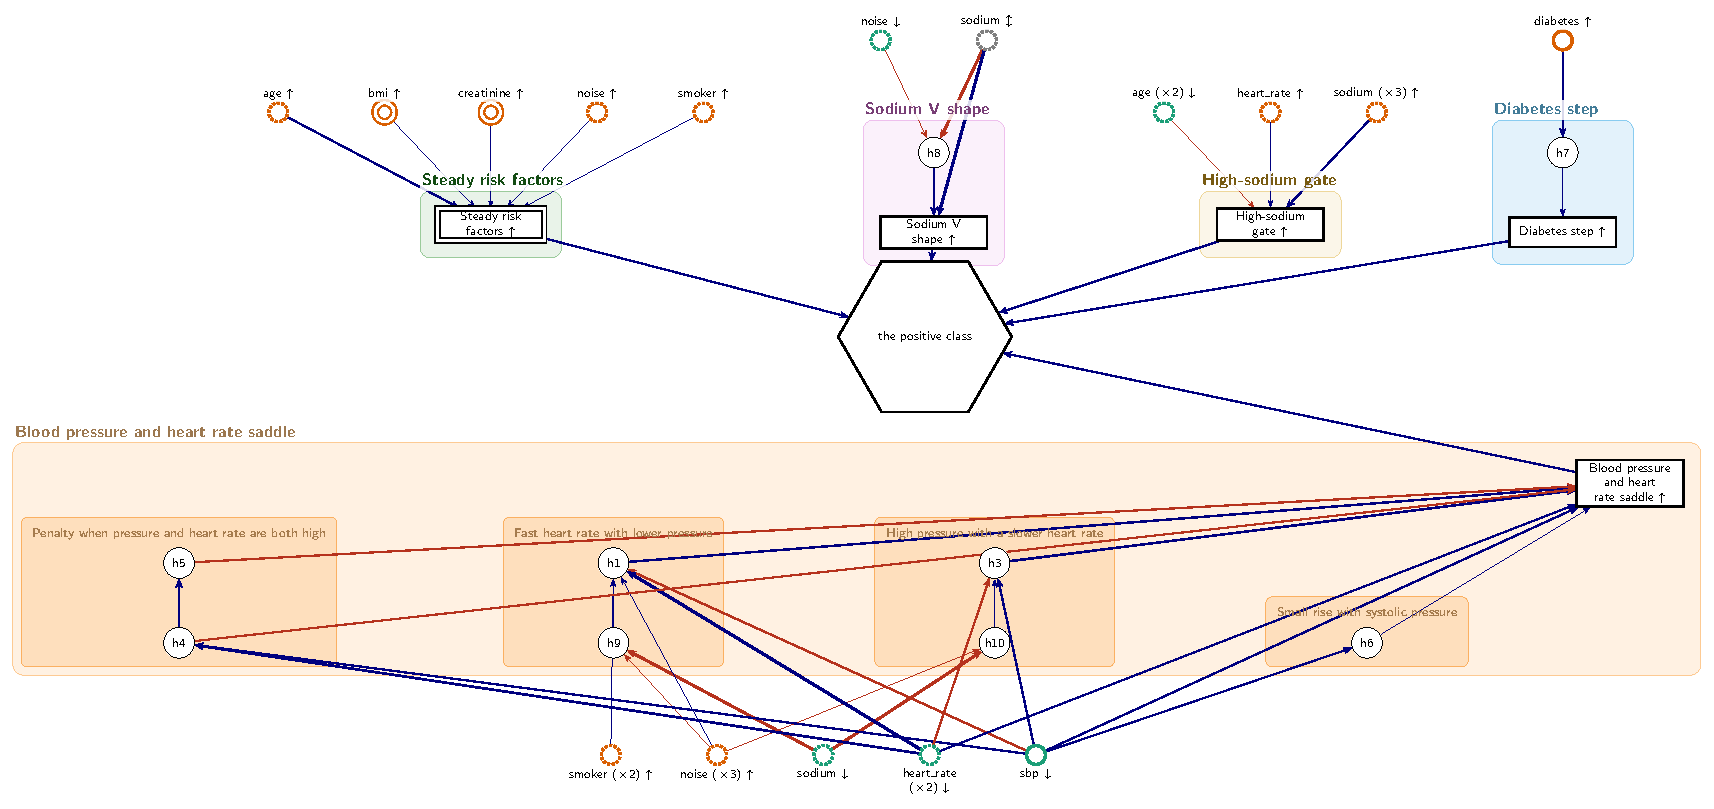
\includegraphics[width=\textheight,height=\netfigheight,keepaspectratio]{figures/exp1/networks/shape-C-explained}
  \caption{Synthetic U and saddle, seed 4: the explained network, every unit nested by part. Shaded boxes: the explanation's parts (inner boxes: sub-parts); white box: a part's output (dashed: a sum standing for the output unit's addition, grey edge). Each input is drawn under every part that reads it (dotted outline, $\times n$: read by $n$ parts); a variable with many levels is drawn once, its edges labelled with their number and weight range (purple: both signs). Orange outline and up arrow: raises the final prediction; teal and down arrow: lowers it; grey and double arrow: depends. Double outline: acts at a fixed rate everywhere (dashed double: on the observed data). Edges as in Figure~\ref{fig:exp1-net-shape-C-raw}.}
  \label{fig:exp1-net-shape-C-explained}
\end{sidewaysfigure}
\clearpage
\clearpage
% XOR
\cleartooddpage
\subsection{XOR}\label{app:exp1-net-xor}
\begin{figure}[!htbp]
  \centering
  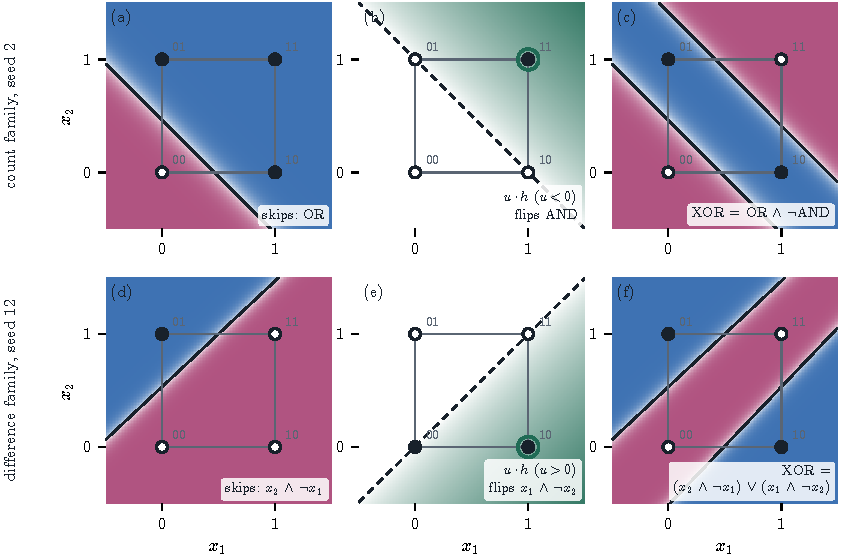
\includegraphics[width=\textwidth,height=0.8\textheight,keepaspectratio]{figures/ch7/xor-gates.pdf}
  \caption{XOR: the gates of the networks of Figure~\ref{fig:ch7-xor-ridge-valley}, the count family (a--c; seed 2) and the difference family (d--f; seed 12). Left: the skip connections alone; middle: the hidden unit's contribution $u\cdot h$ (green: active, darker for larger $|u h|$; dashed: its fold; ringed points: the inputs whose sign it flips); right: the composed score. Shading: blue where the score is positive, magenta where it is negative, pale near 0; solid line: where it is 0. Filled points: inputs where the panel's quantity is positive (middle: where the hidden unit is active).}
  \label{fig:ch7-xor-gates}
\end{figure}
\begin{figure}[!htbp]
  \centering
  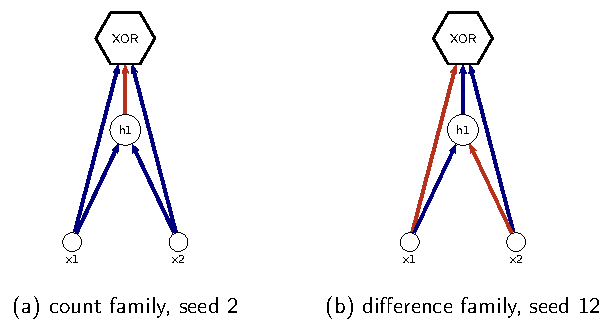
\includegraphics[width=\textwidth,height=0.8\textheight,keepaspectratio]{figures/exp1/networks/xor-raw}
  \caption{XOR: one minimal network of each family, reduced, before any explanation. (a) Count family; (b) difference family. Bottom: the input columns; circles h1, h2, \ldots: hidden units; hexagon: the output. Edges: blue, a positive weight (raises the score); red, a negative weight (lowers it); thicker, a larger weight.}
  \label{fig:exp1-net-xor-raw}
\end{figure}
\clearpage

\end{document}
